\documentclass{article}
\usepackage[utf8]{inputenc}
\usepackage{amssymb}
\usepackage{amsmath}
\usepackage{booktabs}
\usepackage{graphicx}
\usepackage{longtable}



\title{An Assessment of the Effectiveness of Administrative vs. Survey Data for Humanitarian Assistance Targeting}
\author{Colleen O'Donnell, Carlos Guzman, Alec Russin}
\date{December 2020}

\begin{document}

\maketitle
\section{Abstract}

One of the most difficult challenges for governmental bodies and non-profit organizations in the process of giving aid is ensuring the correct population is receiving aid. Aid can be allocated via a number of proxy mechanisms such as geographic or demographic targeting, self or community targeting, or proxy means tests (PMTs). Each of these methods exhibit variation across their implementations, contexts, and performance. PMTs are a common model for poverty targeting. They work by using existing survey data to select a small set of predictors to then survey the eligible population and determine which participants are eligible for the aid. This method typically assigns consumption or expenditure data as a dependent variable to be used as a proxy for poverty and derives a model that weighs factors to predict the poverty level in the eligible population. 
 
In this report, our goal was to develop an econometric expenditure prediction model for refugees in Kenya based on data from the survey “Kenya Socio-economic Profiling Survey of Refugees in Kalobeyei 2018” conducted by the United Nations High Commissioner for Refugees. To do the poverty prediction model, we created a restricted (verifiable variables) and unrestricted dataset (verifiable and unverifiable variables). Ridge, lasso, and elastic net models were run on both datasets and additionally, predicted inclusion and exclusion error rates. Our study found that error rates for both inclusion and exclusion of refugees significantly decreased for the unrestricted dataset in comparison to the restricted. Our findings further support that the survey of all refugees proved beneficial for more accurate aid targeting of the refugee population.

\newpage
\section{Background}
Our report is based on the survey “Kenya Socio-economic Profiling Survey of Refugees in Kalobeyei 2018” conducted by the United Nations High Commissioner for Refugees. Kenya has served as a host site for refugees since 1992, but over the past five years, the Kakuma Refugee Camps have greatly increased in population. In conjunction with the World Bank, the survey was conducted in order to address the current issue that the government of Kenya is currently facing. This issue is the lack of inclusion of the refugee population into national household surveys, which measure various indicators such as the monitoring of poverty. The lack of refugee population inclusion in surveys poses a significant problem given that this population carries substantial impact on the local Kenyan population and national surveys are not accurately capturing differences in poverty between refugees and locals. 

The survey addresses the following criteria: Education, Employment, Household Characteristics, Assets, Access to Services, Vulnerability, Social Cohesion, Consumption and Expenditure Food, Nonfood, Education, and Energy. The survey was conducted using two socio-economic questionnaires, which included a basic and an extended questionnaire. The sample used for the extended questionnaire was obtained by using a systematic random sample. All 6,004 households received the basic questionnaire, but only 1,102 (18.5\%) of households received the extended questionnaire. There is a non-response rate of 2\%, most commonly associated with the lack of an adult household member when the survey was conducted.  

\section{Data}
%% TODO: all data tables in Appendix A
In the appendix Table \ref{table:1} shows descriptive statistics of individual level demographic information on refugees from the Kalobeyei settlement collected through the socioeconomic profiling interview. The refugee population surveyed is predominantly young, uneducated, evenly split by gender, and largely members of female-led households. A significant number of refugees in our sample can speak (65.54\%), while almost half can read (46.30\%) and write (44.97\%). Additionally, less than half have no education (43.86\%), indicating that about 51.14\% of refugees have some level of education. Of those with an education, 27.86\% have a primary education, while 15.64\% have a secondary education. 


In addition to demographic information, we also have information about household assets for the sample refugee population. Table \ref{table:2} in the appendix shows descriptive statistics of all of the assets at a household level. The majority of households own a mosquito net and about half of the households own charcoal. Very few of the refugees own electrically powered items such as a television, a generator, or a refrigerator. Interestingly, 23.49\% of refugees own smartphones, which is significantly more common than other electronically powered items. Less than a quarter of refugees own a table (22.84\%), while very few own a bed (5.41\%). Similarly, 40.01\% of refugees own a toilet. Very few refugees own a mean transportation with bicycles being the most common transportation asset (3.39\%). Furthermore, less than half of the sample owns a toilet and only 19.81\% of refugee households had purchased food in the past seven days. Less than a fourth (19.82\%) of households received food for free, which is the same percentage of households that purchased food in the last seven days. This indicates that those households which purchased food also receive their food for free.

Table \ref{table:3} displays summary statistics of total expenditure per capita and the natural log of total expenditure per capita in Kenyan Shillings (KSH). On average, the refugees in our sample population spent 1,853.32 KSH per capita on a weekly basis. 

%% Box Sync/KenyaPovertyTargetingModel/2progs/C3_RenameVariables2.ipynb
\begin{table}[h]
\centering
\caption{Total Expenditure per Capita}
\begin{tabular}{lrrr}
\toprule
{} &         Mean &          Std &       N \\
\midrule
Expenditure per Capita (KSH) &  1853.32 &  4650.88 &  1090.0 \\
ln (Expenditure per capita)  &     7.07 &     0.87 &  1090.0 \\
\bottomrule
\end{tabular}
\label{table:3}
\end{table}

Summary statistics on total spend per capita broken down by category are shown in Table \ref{table:4} suggesting that refugees spent the majority of their money on food followed by education, while they spent significantly less money on non-food assets and energy sources per week. 
%Box Sync/KenyaPovertyTargetingModel/2progs/Total Spend.ipynb
\begin{table}[h]
\caption{Summary Statistics on Total Spend per Capita by Category}
\centering
\begin{tabular}{lrrr}
\toprule
{} &     Mean &      Std &       N \\
\midrule
Energy Total Spend    &   362.75 &   334.23 &  1090.0 \\
Food Total Spend      &  4829.03 &  2984.09 &  1090.0 \\
Education Total Spend &  2093.95 &  6675.01 &  1090.0 \\
Nonfood Total Spend   &   479.57 &   436.24 &  1090.0 \\
\bottomrule
\end{tabular}
\label{table:4}
\end{table}

Figure 1 provides a density histogram visualization of the natural log of total expenditure per capita with the 25th, 40th, and 50th percentile thresholds. 





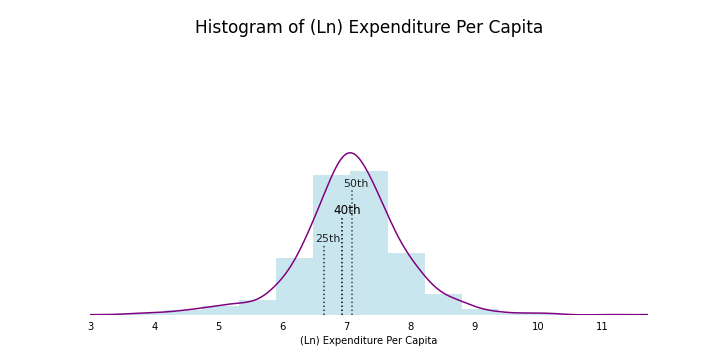
\includegraphics[scale=0.4]{images/figure1.png}




\section{Prediction Model}

Our models are based solely on households chosen for the extended Socio-economic Profiling (SEP) interview. The survey collected information on household characteristics, assets, consumption levels, expenditures, and demographic information about household members. We predict expenditure per capita (in KSH) for all households who received extended SEP interviews between November 2018 and January 2019. Unique identifiers allowed us to merge individual and household level data for further analysis. After cleaning outliers and merging each dataset, we ended with a total of 1,090 households. 

Our approach relies on the ridge regression, the lasso regression, and the elastic net regression. The lasso and elastic net models provide alternative penalty parameters to the ridge model. We fit the models based on our training dataset which is 75\% of the sample (817 households).  We use 10-fold cross validation to select the best alpha parameter and refit the model. We then use the estimated coefficients derived from the training set to predict expenditure using the remaining 25\% of the sample in our validation set (273 households). We were able to assess the discrepancies between the predictions for expenditure by comparing predicted and actual expenditure.


We use the following specification for the ridge regression:


$$\min_{\beta_1,...,\beta_p}\sum_{i=1}^n(y_i-\beta_0-\beta_1x_1-...-\beta_px_p)^2+\lambda \sum_{j=1}^p\beta_j^2$$


where $y_i$ represents ln(expenditure/capita), $\beta_0$ represents the common intercept and $\lambda\sum_{j=1}^p\beta_j^2$ represents the penalty term which penalizes model complexity. 

We use the following specification for the lasso regression:

$$\min_{\beta_1,...,\beta_p}\sum_{i=1}^n(y_i-\beta_0-\beta_1x_1-...-\beta_px_p)^2+\lambda \sum_{j=1}^p|\beta_j|$$

where $y_i$ represents ln(expenditure/capita), $\beta_0$ represents the common intercept and $\lambda\sum_{j=1}^p|\beta_j|$ represents the penalty term which penalizes model complexity. Unlike the ridge regression, the parameter estimates in the lasso regression can be 0 due to the construction of the model. 

We use the following specification for the elastic net regression: 

$$\frac{\sum_{i=1}^n(y_i-x_i^J\hat{\beta})^2}{2n}+\lambda\left( \frac{1-\alpha}{2}\sum_{j=1}^m\hat{\beta^2_j}+\alpha\sum_{j=1}^m|\hat{\beta_j}|\right)$$


where $y_i$ represents ln(expenditure/capita) and\\ $\lambda\left( \frac{1-\alpha}{2}\sum_{j=1}^m\hat{\beta^2_j}+\alpha\sum_{j=1}^m|\hat{\beta_j}|\right)$ represents the penalty term. The elastic net model is a combination of both the ridge and lasso penalties. As a result, the coefficients on the elastic net model should be in between the ridge and lasso models.

\section{Outcome and Prediction Variables}

As described above, we use demographic information and assets at a household level as independent variables while the natural log of expenditure per capita is the dependent variable. We distinguish between verifiable assets and non-verifiable assets in our analysis to take into account potential inaccuracies in survey reporting. We created a restricted dataset which includes demographic variables and assets. Additionally, we created an unrestricted dataset which includes demographic variables and household assets in addition to non-verifiable household assets such as possession of a bank account. See tables \ref{table:2} and \ref{table:7} for summary statistics on all variables in the restricted and unrestricted datasets. While the information in the restricted dataset is typically available in administrative data, the information in the unrestricted dataset is collected by surveying specific populations.

 

We ran the ridge, lasso, and elastic net models on both the restricted and unrestricted datasets. See tables \ref{table:MergedRestrict} and \ref{table:MergedUnrestrict} for our results. We replace all missing values with NAs so that all households can receive a predicted expenditure score. Our goal is to determine to what extent humanitarian assistance targeting improves if we use administrative data such as the restricted set compared to surveying the refugee population based on our unrestricted set. 

\section{Prediction Accuracy}

We use two error metrics to assess the accuracy of our models. Exclusion error represents eligible households who fail to receive cash transfers. On the other hand, the inclusion error metric reflects the percentage of refugees who receive transfers given they were ineligible for the program. We report the exclusion and inclusion errors at the 25, 40, and 50th percentiles of the expenditure per capita distribution in Table \ref{table:5} and Table \ref{table:6}. 

%%Box Sync/KenyaPovertyTargetingModel/3analysis/Error Rate Chart.ipynb

\begin{table}[h]
    \caption{Exclusion Error of Expenditure per Capita as Percentages}
    \centering
    \begin{tabular}{lllllll}
        \toprule
        {} & \multicolumn{3}{c}{Restricted} & \multicolumn{3}{c}{Unrestricted}\\
        \cmidrule(lr){2-4} \cmidrule(lr){5-7} \\
        Percentile & Lasso & Ridge & Elastic Net  & Lasso & Ridge & Elastic Net \\
        \midrule
        25\%        &   60.29 &  61.76 &        64.71  &   48.52 &  42.64 &        45.59\\
        40\%        &   48.62 &  44.95 &        45.87  &   35.78 &  31.19 &        32.11\\
        50\%        &   36.76 &  34.56 &        33.82  &   24.26 &  24.26 &        25.00\\
        \bottomrule
    \end{tabular}
    \label{table:5}
\end{table}


For the restricted models based on the 50th percentile of expenditure per capita, the elastic net model displays the lowest exclusion error rate of 33.82\% compared to the ridge model with a 34.55\% exclusion error and the lasso model with a 36.76\% exclusion error. However, the unrestricted dataset provides substantial improvement in exclusion error rates relative to the restricted datasets. The unrestricted models based on the 50th percentile of expenditure per capita suggest that the ridge and lasso models have the lowest exclusion error of 24.26\% followed by the elastic net model with a 25.00\%  exclusion error. We show that the different penalty terms in the regression equation make little difference to prediction performance. 

%%Box Sync/KenyaPovertyTargetingModel/3analysis/Error Rate Chart.ipynb

\begin{table}[h]
\caption{Inclusion Error of Expenditure per Capita as Percentages}
    \centering
    \begin{tabular}{lllllll}
        \toprule
        {} & \multicolumn{3}{c}{Restricted} & \multicolumn{3}{c}{Unrestricted}\\
        \cmidrule(lr){2-4} \cmidrule(lr){5-7} \\
        Percentile & Lasso & Ridge & Elastic Net  & Lasso & Ridge & Elastic Net \\
        \midrule
        25\% &61.35&76.36&78.57&45.21		&	59.79	&		46.10\\
40\%&		53.34	&		56.52	&		57.86& 44.44	&		40.48	&		43.95\\
50\%	&	47.24	&		44.03&			43.40 &	39.05	&		30.41 	&		40.00\\
        \bottomrule
    \end{tabular}
    \label{table:6}
\end{table}



At the 50th percentile for the restricted set, the elastic net model has the smallest inclusion error of 43.40\%, followed by the 44.03\% inclusion error in the ridge model and the 47.24\% inclusion error in the lasso model. On the other hand, the unrestricted models based on the 50th percentile of expenditure per capita display slightly lower error rates. The ridge model has a 30.41\% inclusion error while the lasso and elastic net have inclusion errors of 39.05\% and 40.00\% respectively.

\section{Conclusion}

We conclude that surveying the refugee population reduces inclusion and exclusion error in humanitarian assistance targeting in comparison to relying on administrative data. Our models based on administrative data exhibit higher error rates relative to Altındag et al.’s research. As a result, it may be necessary to explore whether there are other variables that should be included in our administrative dataset to improve prediction accuracy. Another explanation for these results is that the data necessary to target aid is population specific. It may be effective to rely on survey data to target assistance to refugees in the Kalobeyei settlement while administrative data is sufficient to target other populations.

Future research should explore which variables in the survey dataset are heavily weighted and thus contributing to significantly lower error rates in the survey data relative to the administrative data. Our models may also be better at targeting specific subgroups in the refugee population relative to others. As a result, researchers should also consider whether the prediction accuracy improves amongst population subgroups. 



 \newpage
 \section{References}

1. Altindag, Onur, et al. “Targeting Humanitarian Aid Using Administrative Data: Model Design and Validation.” SSRN Electronic Journal, 2019, doi:10.2139/ssrn.3444974.

2. “Kenya Socio-economic Profiling Survey of Refugees in Kalobeyei 2018.” United Nations High Commissioner for Refugees, 2020.

3. “Understanding the Socio-economic Conditions of Refugees in Kalobeyei, Kenya.” United Nations High Commissioner for Refugees, 2018.  

\newpage
\appendix

\renewcommand\thefigure{\thesection.\arabic{table}} 

\section{ppendix}
\setcounter{table}{0}
%Box Sync/KenyaPovertyTargetingModel/2progs/Total Spend.ipynb
\begin{longtable}{lrrr}
\caption{Descriptive Stats of Individual  Demographic Information}
\label{table:1}


\\\hline
{} &  Mean &   Std &       N \\
\hline
\endhead

\hline
\endfoot
Head Female                              &  0.66 &  0.48 &  1100.0 \\
Share Female                             &  0.49 &  0.26 &  1100.0 \\
\% Members Aged 0-4                       &  0.19 &  0.17 &  1100.0 \\
\% Members Aged 5-9                       &  0.19 &  0.17 &  1100.0 \\
\% Members Aged 10-14                     &  0.15 &  0.16 &  1100.0 \\
\% Members Aged 15-24                     &  0.22 &  0.25 &  1100.0 \\
\% Members Aged 25-49                     &  0.22 &  0.23 &  1100.0 \\
\% Members Over Age 50                    &  0.01 &  0.07 &  1100.0 \\
\% Male Members Aged 10-19                &  0.16 &  0.20 &  1100.0 \\
\% Female Members Aged 10-19              &  0.12 &  0.15 &  1100.0 \\
\% Male Members Aged 20-49                &  0.16 &  0.27 &  1100.0 \\
\% Female Members Aged 20-49              &  0.15 &  0.14 &  1100.0 \\
\% Members with No Education              &  0.44 &  0.44 &  1100.0 \\
\% Members with Early Childhood Education &  0.00 &  0.03 &  1100.0 \\
\% Members with Primary Education         &  0.28 &  0.39 &  1100.0 \\
\% Members with Secondary Education       &  0.16 &  0.31 &  1100.0 \\
\% Members with Vocational Education      &  0.02 &  0.13 &  1100.0 \\
\% Members with University Education      &  0.02 &  0.11 &  1100.0 \\
\% Members with Other Education           &  0.02 &  0.11 &  1100.0 \\
\% Members who Speak                      &  0.65 &  0.47 &  1100.0 \\
\% Members who Read                       &  0.46 &  0.45 &  1100.0 \\
\% Members who Write                      &  0.45 &  0.44 &  1100.0 \\
\end{longtable}
%Box Sync/KenyaPovertyTargetingModel/3analysis/Analysis.ipynb
\begin{longtable}{lrrr}
\caption{Descriptive Stats of  Restricted Data for Household Level}
\label{table:2}

\\\hline
{} &  Mean &   Std &       N \\
\hline
\endhead

\hline
\endfoot


Number of Dwellings                      &  1.32 &  0.56 &  1090.0 \\
Number of Habitable Rooms                &  1.40 &  0.67 &  1090.0 \\
Owns a Radio                             &  0.05 &  0.22 &  1090.0 \\
Owns a Television                        &  0.01 &  0.09 &  1090.0 \\
Owns a Satelite Dish                     &  0.01 &  0.08 &  1090.0 \\
Owns a Smartphone                        &  0.23 &  0.42 &  1090.0 \\
Owns a Refrigerator                      &  0.00 &  0.05 &  1090.0 \\
Owns a Table                             &  0.23 &  0.42 &  1090.0 \\
Owns a Bed                               &  0.05 &  0.23 &  1090.0 \\
Owns a Mattress                          &  0.32 &  0.47 &  1090.0 \\
Owns a Mosquito Net                      &  0.93 &  0.26 &  1090.0 \\
Owns a Fan                               &  0.01 &  0.07 &  1090.0 \\
Owns a Bicycle                           &  0.03 &  0.18 &  1090.0 \\
Owns a Motorcycle                        &  0.02 &  0.12 &  1090.0 \\
Owns a Generator                         &  0.00 &  0.05 &  1090.0 \\
Owns Solar Panels                        &  0.06 &  0.23 &  1090.0 \\
Owns Kerosene Stove                      &  0.04 &  0.19 &  1090.0 \\
Owns Charcoal                            &  0.59 &  0.49 &  1090.0 \\
Owns a Wheelbarrow                       &  0.04 &  0.19 &  1090.0 \\
Owns Iron Fencing                        &  0.01 &  0.10 &  1090.0 \\
Owns Farm Animals                        &  0.20 &  0.40 &  1090.0 \\
Head of Household - Female               &  0.66 &  0.47 &  1090.0 \\
Share of Household - Female              &  0.49 &  0.26 &  1090.0 \\
\% Members Aged 0-4                       &  0.19 &  0.17 &  1090.0 \\
\% Members Aged 5-9                       &  0.19 &  0.17 &  1090.0 \\
\% Members Aged 10-14                     &  0.15 &  0.16 &  1090.0 \\
\% Members Aged 15-24                     &  0.22 &  0.25 &  1090.0 \\
\% Members Aged 25-49                     &  0.22 &  0.23 &  1090.0 \\
\% Members Over Age 50                    &  0.01 &  0.07 &  1090.0 \\
\% Male Members Aged 10-19                &  0.16 &  0.20 &  1090.0 \\
\% Female Members Aged 10-19              &  0.12 &  0.15 &  1090.0 \\
\% Male Members Aged 20-49                &  0.16 &  0.26 &  1090.0 \\
\% Female Members Aged 20-49              &  0.16 &  0.14 &  1090.0 \\
\% Members with No Education              &  0.45 &  0.44 &  1090.0 \\
\% Members with Early Childhood Education &  0.00 &  0.03 &  1090.0 \\
\% Members with Primary Education         &  0.28 &  0.39 &  1090.0 \\
\% Members with Secondary Education       &  0.16 &  0.31 &  1090.0 \\
\% Members with Vocational Education      &  0.02 &  0.13 &  1090.0 \\
\% Members with University Education      &  0.02 &  0.11 &  1090.0 \\
\% Members with Other Education           &  0.02 &  0.11 &  1090.0 \\
Owns Lighting Source                     &  2.43 &  1.56 &  1090.0 \\
Owns Floor Material                      &  1.32 &  0.82 &  1090.0 \\
Owns Roof Material                       &  1.04 &  0.33 &  1090.0 \\
Owns Wall Material                       &  1.29 &  0.67 &  1090.0 \\
Toilet Type                              &  2.64 &  0.98 &  1090.0 \\
Owns Toilet                              &  0.40 &  0.49 &  1090.0 \\
Receives Free Food                       &  0.20 &  0.40 &  1090.0 \\
Household Purchased Food in last 7 days  &  0.20 &  0.40 &  1090.0 \\
\end{longtable}


%%Box Sync/KenyaPovertyTargetingModel/3analysis/Analysis.ipynb
\begin{longtable}{lrrr}
\caption{Descriptive Stats of  Unestricted Data for Household Level}
\label{table:7}
\\\hline
{} &  Mean &   Std &       N \\
\hline
\endhead

\hline
\endfoot
Size of Household                                  &  5.76 &  3.08 &  1090.0 \\
Head of Household - Female                         &  0.66 &  0.47 &  1090.0 \\
Share of Household - Female                        &  0.49 &  0.26 &  1090.0 \\
\% Members Aged 0-4                                 &  0.19 &  0.17 &  1090.0 \\
\% Members Aged 5-9                                 &  0.19 &  0.17 &  1090.0 \\
\% Members Aged 10-14                               &  0.15 &  0.16 &  1090.0 \\
\% Members Aged 15-24                               &  0.22 &  0.25 &  1090.0 \\
\% Members Aged 25-49                               &  0.22 &  0.23 &  1090.0 \\
\% Members Over Age 50                              &  0.01 &  0.07 &  1090.0 \\
\% Male Members Aged 10-19                          &  0.16 &  0.20 &  1090.0 \\
\% Female Members Aged 10-19                        &  0.12 &  0.15 &  1090.0 \\
\% Male Members Aged 20-49                          &  0.16 &  0.26 &  1090.0 \\
\% Female Members Aged 20-49                        &  0.16 &  0.14 &  1090.0 \\
\% Members Age Not Available                        &  0.02 &  0.10 &  1090.0 \\
\% Members with No Education                        &  0.45 &  0.44 &  1090.0 \\
\% Members with Early Childhood Education           &  0.00 &  0.03 &  1090.0 \\
\% Members with Primary Education                   &  0.28 &  0.39 &  1090.0 \\
\% Members with Secondary Education                 &  0.16 &  0.31 &  1090.0 \\
\% Members with Vocational Education                &  0.02 &  0.13 &  1090.0 \\
\% Members with University Education                &  0.02 &  0.11 &  1090.0 \\
\% Members with Other Education                     &  0.02 &  0.11 &  1090.0 \\
\% Member who Speak                                 &  0.66 &  0.47 &  1090.0 \\
\% Members who Read                                 &  0.47 &  0.44 &  1090.0 \\
\% Members who Write                                &  0.46 &  0.44 &  1090.0 \\
Household Purchased Food in last 7 days            &  0.20 &  0.40 &  1090.0 \\
Receives Free Food                                 &  0.20 &  0.40 &  1090.0 \\
Size of Family 1                                   &  5.34 &  2.87 &  1090.0 \\
Size of Family 2                                   &  0.37 &  1.13 &  1090.0 \\
Size of Family 3                                   &  0.04 &  0.36 &  1090.0 \\
Size of Family 4                                   &  0.01 &  0.11 &  1090.0 \\
Size of Family 5                                   &  0.00 &  0.00 &  1090.0 \\
Number of Dwellings                                &  1.32 &  0.56 &  1090.0 \\
Number of Habitable Rooms                          &  1.40 &  0.67 &  1090.0 \\
Number of Dwellings                                &  1.32 &  0.82 &  1090.0 \\
Number of Habitable Rooms                          &  1.04 &  0.33 &  1090.0 \\
Owns Floor Material                                &  1.29 &  0.67 &  1090.0 \\
Owns Roof Material                                 &  1.04 &  0.29 &  1090.0 \\
Owns Wall Material                                 &  2.64 &  0.98 &  1090.0 \\
Drinking Water Source                              &  2.43 &  1.56 &  1090.0 \\
Toilet Type                                        &  0.00 &  0.00 &  1090.0 \\
Lighting Source                                    &  1.82 &  0.62 &  1090.0 \\
Household Members Per Room                         &  1.82 &  0.62 &  1090.0 \\
Livelihood Coping Strategy Index                   &  0.06 &  1.68 &  1090.0 \\
Asset index based on PCA                           &  1.90 &  0.00 &  1090.0 \\
International Poverty Line (2011)                  &  1.82 &  0.62 &  1090.0 \\
Being below the International Poverty line (201... &  0.16 &  0.21 &  1090.0 \\
Poverty severity from cons aggregate and intern... &  0.07 &  0.12 &  1090.0 \\
Owns Radio                                         &  0.05 &  0.22 &  1090.0 \\
Owns Television                                    &  0.01 &  0.09 &  1090.0 \\
Insufficient Drinking Water                        &  0.66 &  0.47 &  1090.0 \\
Owns a Satelite Dish                               &  0.01 &  0.08 &  1090.0 \\
Owns a Smartphone                                  &  0.23 &  0.42 &  1090.0 \\
Owns a Refrigerator                                &  0.00 &  0.05 &  1090.0 \\
Owns a Table                                       &  0.23 &  0.42 &  1090.0 \\
Owns a Bed                                         &  0.05 &  0.23 &  1090.0 \\
Owns a Mattress                                    &  0.32 &  0.47 &  1090.0 \\
Owns a Mosquito Net                                &  0.93 &  0.26 &  1090.0 \\
Owns a Fan                                         &  0.01 &  0.07 &  1090.0 \\
Owns a Bicycle                                     &  0.03 &  0.18 &  1090.0 \\
Owns a Motorcycle                                  &  0.02 &  0.12 &  1090.0 \\
Owns a Generator                                   &  0.00 &  0.05 &  1090.0 \\
Owns Solar Panels                                  &  0.06 &  0.23 &  1090.0 \\
Owns Kerosene Stove                                &  0.04 &  0.19 &  1090.0 \\
Owns Charcoal                                      &  0.59 &  0.49 &  1090.0 \\
Owns a Wheelbarrow                                 &  0.04 &  0.19 &  1090.0 \\
Owns Iron Fencing                                  &  0.01 &  0.10 &  1090.0 \\
Owns Farm Animals                                  &  0.20 &  0.40 &  1090.0 \\
Relatives Aborad                                   &  0.13 &  0.33 &  1090.0 \\
Relatives Outside Kenya                            &  0.10 &  0.30 &  1090.0 \\
Owns Bank Account                                  &  0.28 &  0.45 &  1090.0 \\
Borrowed from Sources Past 12 Months               &  0.14 &  0.35 &  1090.0 \\
Borrowed from Bank Past 12 Months                  &  0.02 &  0.13 &  1090.0 \\
Borrowed from Community Past 12 Months             &  0.03 &  0.17 &  1090.0 \\
Borrowed from Family/Friends Past 12 Months        &  0.11 &  0.31 &  1090.0 \\
Remittances from Aborad                            &  0.06 &  0.23 &  1090.0 \\
Purchased Insurance                                &  0.01 &  0.07 &  1090.0 \\
Sell Goods Lack of Food                            &  0.16 &  0.37 &  1090.0 \\
Health and Education Reducation Lack Food          &  0.14 &  0.35 &  1090.0 \\
Sell Assets Lack Food                              &  0.09 &  0.29 &  1090.0 \\
Spend Savings Lack Food                            &  0.22 &  0.42 &  1090.0 \\
Borrowed Money Lack Food                           &  0.33 &  0.47 &  1090.0 \\
Sell House/Land Lack Food                          &  0.02 &  0.13 &  1090.0 \\
Withdraw Children From School Lack Food            &  0.04 &  0.19 &  1090.0 \\
Sells Animals Lack Food                            &  0.05 &  0.22 &  1090.0 \\
Sell Last Female Animal Lack Food                  &  0.04 &  0.19 &  1090.0 \\
 Beg Lack Food                                     &  0.13 &  0.33 &  1090.0 \\
Shares Toilet                                      &  0.40 &  0.49 &  1090.0 \\

\bottomrule
\end{longtable}
\begin{longtable}{lrrr}


\caption{Model Coefficients for Restricted data set}
\label{table:MergedRestrict}

\\\hline
{} &  Ridge  &  Lasso  &  Elastic Net  \\
\hline
\endhead

\hline
\endfoot

number\_dwellings &              -0.07 &               -0.02 &                     -0.04 \\
number\_habitablerooms &              -0.05 &               -0.05 &                     -0.08 \\
own\_radio\_Yes &               0.16 &                0.16 &                      0.18 \\
own\_television\_Yes &               0.05 &                0.00 &                      0.00 \\
own\_satelitedish\_Yes &               0.25 &                0.34 &                      0.00 \\
own\_smartphone\_Yes &               0.07 &                0.00 &                      0.03 \\
own\_refrigerator\_Yes &               0.46 &                0.00 &                      0.00 \\
own\_table\_Yes &               0.07 &                0.06 &                      0.08 \\
own\_bed\_Yes &               0.15 &                0.05 &                      0.07 \\
own\_mattress\_Yes &               0.06 &                0.02 &                      0.05 \\
own\_mosquitonet\_Yes &               0.02 &                0.00 &                      0.00 \\
own\_fan\_Yes &               0.08 &                0.00 &                      0.00 \\
own\_bicycle\_Yes &               0.14 &                0.08 &                      0.04 \\
own\_motorcycle\_Yes &               0.01 &                0.00 &                      0.00 \\
own\_generator\_Yes &              -0.24 &                0.00 &                      0.00 \\
own\_solarpanels\_Yes &              -0.00 &               -0.00 &                     -0.00 \\
own\_kerosenestove\_Yes &               0.18 &                0.08 &                      0.10 \\
own\_charcoaljiko\_Yes &               0.12 &                0.10 &                      0.14 \\
own\_wheelbarrow\_Yes &               0.16 &                0.05 &                      0.05 \\
own\_ironfencing\_Yes &               0.10 &               -0.00 &                     -0.00 \\
own\_farmanimals\_Yes &              -0.03 &               -0.00 &                     -0.00 \\
headFemale &              -0.04 &               -0.00 &                     -0.02 \\
shareFemale &              -0.08 &               -0.02 &                     -0.03 \\
shareAgeZeroToFour &              -0.33 &               -0.24 &                     -0.18 \\
shareAgeFiveToNine &              -0.32 &               -0.09 &                     -0.03 \\
shareAgeTenToFourteen &              -0.24 &               -0.00 &                     -0.00 \\
shareAgeFifteenToTwentyfour &               0.26 &                0.51 &                      0.51 \\
shareAgeTwentyfivetofourtynine &               0.14 &                0.31 &                      0.33 \\
shareAgeFiftyPlus &               0.10 &                0.00 &                      0.00 \\
shareMaleAgeTenToNineteen &               0.01 &                0.00 &                      0.00 \\
shareFemaleAgeTenToNineteen &              -0.02 &               -0.00 &                     -0.00 \\
shareMaleAgeTwentytoFourtynine &               0.15 &                0.34 &                      0.29 \\
shareFemaleAgeTwentytoFourtynine &               0.41 &                0.44 &                      0.33 \\
shareWithNoEducation &              -0.17 &               -0.30 &                     -0.36 \\
shareWithEarlyChildhood &              -0.70 &               -0.36 &                     -0.00 \\
shareWithPrimary &              -0.10 &               -0.20 &                     -0.28 \\
shareWithSecondary &               0.07 &                0.00 &                     -0.00 \\
shareWithVocational &               0.36 &                0.15 &                      0.00 \\
shareWithUniversity &               0.33 &                0.00 &                      0.00 \\
shareWithOther &               0.13 &                0.00 &                     -0.00 \\
lighting\_source &              -0.01 &               -0.01 &                     -0.03 \\
floor\_material &               0.02 &                0.00 &                      0.02 \\
roof\_material &               0.00 &               -0.00 &                     -0.00 \\
wall\_material &              -0.06 &               -0.02 &                     -0.06 \\
toilet\_type &               0.01 &                0.00 &                      0.03 \\
share\_toilet\_Yes &               0.06 &                0.01 &                      0.06 \\
foodwasfree\_Yes &              -0.03 &               -0.00 &                     -0.00 \\
hh\_purchasedfood7d\_Yes &              -0.03 &               -0.00 &                     -0.00 \\

\end{longtable}
\begin{longtable}{lrrr}

\caption{Model Coefficients for Unrestricted data set}
\label{table:MergedUnrestrict}
\\\hline
{} &  Ridge  &  Lasso  &  Elastic Net  \\
\hline
\endhead

\hline
\endfoot
size &               -0.02 &               -0.04 &                     -0.07 \\
headFemale &               -0.01 &               -0.00 &                      0.00 \\
shareFemale &               -0.07 &               -0.06 &                     -0.07 \\
shareAgeZeroToFour &               -0.19 &               -0.20 &                     -0.07 \\
shareAgeFiveToNine &               -0.09 &               -0.00 &                     -0.00 \\
shareAgeTenToFourteen &               -0.09 &               -0.00 &                      0.00 \\
shareAgeFifteenToTwentyfour &                0.19 &                0.31 &                      0.28 \\
shareAgeTwentyfivetofourtynine &               -0.00 &                0.00 &                      0.00 \\
shareAgeFiftyPlus &               -0.03 &               -0.00 &                     -0.00 \\
shareMaleAgeTenToNineteen &                0.04 &                0.00 &                      0.00 \\
shareFemaleAgeTenToNineteen &                0.03 &               -0.00 &                      0.00 \\
shareMaleAgeTwentytoFourtynine &                0.05 &                0.04 &                      0.00 \\
shareFemaleAgeTwentytoFourtynine &                0.23 &                0.00 &                      0.00 \\
shareAgeNaN &               -0.18 &               -0.07 &                     -0.00 \\
shareWithNoEducation &               -0.09 &               -0.06 &                     -0.18 \\
shareWithEarlyChildhood &               -0.70 &               -0.25 &                     -0.00 \\
shareWithPrimary &               -0.07 &               -0.00 &                     -0.16 \\
shareWithSecondary &                0.07 &                0.17 &                      0.03 \\
shareWithVocational &                0.30 &                0.31 &                      0.00 \\
shareWithUniversity &                0.29 &                0.09 &                      0.00 \\
shareWithOther &                0.10 &                0.00 &                      0.00 \\
shareSpeaks &               -0.07 &               -0.06 &                     -0.04 \\
shareReads &                0.02 &                0.00 &                      0.05 \\
shareWrites &                0.02 &                0.00 &                      0.00 \\
hh\_purchasedfood7d\_Yes &               -0.02 &               -0.00 &                     -0.00 \\
foodwasfree\_Yes &               -0.02 &               -0.00 &                     -0.00 \\
familysize1 &               -0.02 &               -0.00 &                     -0.00 \\
familysize2 &               -0.01 &                0.00 &                      0.01 \\
familysize3 &               -0.04 &               -0.00 &                     -0.01 \\
familysize4 &               -0.03 &               -0.00 &                     -0.00 \\
familysize5 &                0.00 &                0.00 &                      0.00 \\
number\_dwellings &                0.02 &                0.00 &                      0.12 \\
number\_habitablerooms &               -0.00 &                0.00 &                     -0.00 \\
floor\_material &                0.04 &                0.02 &                      0.06 \\
roof\_material &                0.04 &                0.00 &                      0.02 \\
wall\_material &               -0.06 &               -0.02 &                     -0.06 \\
drikingwater\_source &                0.04 &                0.00 &                      0.00 \\
toilet\_type &                0.01 &                0.00 &                      0.02 \\
lighting\_source &               -0.01 &               -0.01 &                     -0.03 \\
rentpaid\_shillings &                0.00 &                0.00 &                      0.00 \\
crowdindex\_room &                0.02 &                0.05 &                      0.03 \\
LCS\_index &                0.02 &                0.00 &                      0.04 \\
asset\_idx &                0.02 &                0.04 &                      0.05 \\
pline\_ipl &                0.00 &                0.00 &                      0.00 \\
poorIPL &                0.02 &                0.00 &                      0.03 \\
pgi &               -0.56 &               -1.15 &                     -0.94 \\
spg &               -0.57 &               -0.00 &                     -0.00 \\
own\_radio\_Yes &                0.12 &                0.05 &                      0.04 \\
own\_television\_Yes &               -0.03 &                0.00 &                     -0.00 \\
drinkingwater\_insufficientquanities\_Yes &               -0.00 &               -0.00 &                     -0.00 \\
own\_satelitedish\_Yes &                0.15 &                0.00 &                      0.00 \\
own\_smartphone\_Yes &                0.03 &                0.00 &                     -0.00 \\
own\_refrigerator\_Yes &                0.44 &                0.00 &                      0.00 \\
own\_table\_Yes &                0.05 &                0.00 &                      0.01 \\
own\_bed\_Yes &                0.13 &                0.02 &                      0.00 \\
own\_mattress\_Yes &                0.03 &                0.00 &                     -0.00 \\
own\_mosquitonet\_Yes &                0.03 &                0.00 &                      0.00 \\
own\_fan\_Yes &                0.08 &                0.00 &                      0.00 \\
own\_bicycle\_Yes &                0.12 &                0.02 &                      0.00 \\
own\_motorcycle\_Yes &               -0.08 &               -0.00 &                     -0.00 \\
own\_generator\_Yes &               -0.15 &               -0.00 &                     -0.00 \\
own\_solarpanels\_Yes &               -0.06 &               -0.00 &                     -0.11 \\
own\_kerosenestove\_Yes &                0.11 &                0.00 &                      0.00 \\
own\_charcoaljiko\_Yes &                0.09 &                0.04 &                      0.07 \\
own\_wheelbarrow\_Yes &                0.16 &                0.03 &                      0.00 \\
own\_ironfencing\_Yes &                0.07 &               -0.00 &                     -0.00 \\
own\_farmanimals\_Yes &               -0.02 &               -0.00 &                     -0.00 \\
relatives\_abroad\_Yes &                0.04 &                0.00 &                      0.00 \\
relatives\_outsidekenya\_Yes &                0.09 &                0.01 &                      0.05 \\
 own\_bankaccount\_Yes &               -0.13 &               -0.10 &                     -0.17 \\
borrowedfrom\_sources12mo\_Yes &                0.05 &                0.07 &                      0.12 \\
borrowedfrom\_bank12mo\_Yes &                0.11 &               -0.00 &                     -0.00 \\
borrowedfrom\_community\_Yes &                0.12 &                0.00 &                      0.00 \\
borrowedfrom\_familyorfriends12mo\_Yes &               -0.02 &                0.00 &                      0.00 \\
remittances\_abroad\_Yes &                0.04 &                0.00 &                      0.00 \\
purchased\_insurance\_Yes &               -0.16 &               -0.00 &                     -0.00 \\
sellhhgoods\_lackfood\_Yes &                0.09 &                0.03 &                      0.08 \\
healthandeduc\_reduction\_Yes &                0.11 &                0.13 &                      0.16 \\
sellassets\_lackfood\_Yes &                0.05 &                0.00 &                      0.00 \\
spendsavings:lackfood\_Yes &                0.01 &                0.00 &                      0.01 \\
borrowmoneyfood\_lackfood\_Yes &                0.01 &                0.00 &                      0.00 \\
sellhouseland\_lackfood\_Yes &               -0.12 &               -0.00 &                     -0.00 \\
withdrawchildrenschool\_lackfood\_Yes &                0.01 &                0.00 &                      0.00 \\
sellanimals:lackfood\_Yes &               -0.18 &               -0.13 &                     -0.16 \\
sellfemaleanimal\_last\_Yes &               -0.15 &               -0.04 &                     -0.06 \\
beg\_lackfood\_Yes &                0.01 &               -0.00 &                      0.00 \\
share\_toilet\_Yes &                0.04 &                0.00 &                      0.01 \\
\end{longtable}


\end{document}
